\documentclass{article}
\usepackage{graphicx} % Required for inserting images
\usepackage{authblk} % Required for author affiliations
\usepackage{indentfirst} % Indent first paragraph of sections
\usepackage{amssymb} % For mathematical symbols
\usepackage{amsthm} % For theorem environments
\usepackage{amsmath} % For advanced math typesetting
\usepackage[hidelinks]{hyperref}
\usepackage{enumitem}
\usepackage{pgfplots} % For plots
\usetikzlibrary{arrows.meta,calc}
\pgfplotsset{compat=1.18} % Set compatibility level
\usepackage{tikz} % For drawing shapes
\newtheorem{theorem}{Theorem}
\newtheorem{corollary}{Corollary}[theorem]
\newtheorem{lemma}[theorem]{Lemma}
\newtheorem{definition}{Definition}
\newtheorem{problem}{Problem}
\newtheorem{solution}{Solution}
\newtheorem*{example}{Example}
\newtheorem{remark}{Remark}
\newtheorem{proposition}{Proposition}
\reversemarginpar
\begin{document}
%------- Title page   -----------
\title{MATH 223: Linear Algebra}
\author{William Homier}
\affil[1]{McGill University Physics, 3600 Rue University, Montréal, QC H3A 2T8, Canada}
\date{January \(5^{th}\), 2026}
\setcounter{Maxaffil}{0}
\renewcommand\Affilfont{\itshape\small}
\maketitle

%------- Abstract -----------
\noindent\rule{\textwidth}{0.4pt}
\thispagestyle{empty}
\begin{abstract}

\end{abstract}
\noindent\rule{\textwidth}{0.4pt}
\clearpage

%------- Table of Contents -----------
\thispagestyle{empty}
\hypersetup{
    citecolor=black,
    filecolor=black,
    linkcolor=black,
    urlcolor=black
}
\tableofcontents
\clearpage

%------- introduction -----------
\setcounter{page}{1}
\section{Introduction}

\section{Prerequisite knowledge}
\subsection{Notation}
\subsubsection{Sets}
Sets are a grouping of objects.
\begin{center}
\begin{tabular}{c|p{6cm}|p{5cm}}
Set & Meaning & Examples \\
\hline
$\mathbb{N}$ & The set of natural numbers & (0, 1, 2, 3, ...)\\
$\mathbb{Z}$ & The set of integers & (..., -3, -2, -1, 0, 1, 2, 3, ...)\\
$\mathbb{Q}$ & The set of rational numbers & \(\mathbb{Q} = {\frac{a}{b}\:|\:\forall a,b \in \mathbb{Z}\:and\:b \neq 0}\)\\
$\mathbb{R}$ & The set of all rational and all irrational numbers & \((...,-1,0,\frac{1}{4},1,1000,...)\)\\
$\mathbb{C}$ & The set of all complex numbers & \(\mathbb{C} = \{x + iy\:|\:x,y \in \mathbb{R}\:and\:i \subseteq \sqrt{-1}\}\).\\
\end{tabular}
\end{center}

We have the following relationships between sets:
\[\mathbb{N} \subseteq \mathbb{Z} \subseteq \mathbb{Q} \subseteq \mathbb{R} \subseteq \mathbb{C}\]
\subsubsection{Symbols}
\begin{center}
\begin{tabular}{c|l}
Symbol & Meaning \\
\hline
$\subseteq$ & is a subset of or equal to \\
$\subset$ & is a strict subset of \\
$\in$ & is an element of \\
$\forall$ & for all \\
$\exists$ & there exists \\
$\emptyset$ & empty set \\
$\Rightarrow$ & implies \\
$\Leftrightarrow$ & if and only if
\end{tabular}
\end{center}

\subsection{Complex Algebra}
\subsubsection{Complex Numbers}
A complex number is of the form: \(z = x + iy\) where \(x,y \in \mathbb{R}\) and \(i\) is the imaginary unit such that \(i^2 + 1 = 0\).
\begin{definition}[Powers of \(i\)]
\begin{tabular}{c|cccccc}
k & 0 & 1 & 2 & 3 & 4 & 5 \\
\hline
$i^k$ & 1 & i & -1 & -i & 1 & i
\end{tabular}
\end{definition}
\begin{theorem}[Fundamental Theorem of Algebra]
    Any complex polynomial\footnote{Polynomial is a function such as: \(f = a_n x^n + a_{n-1}x^{n-1} + ... + a_1 x + a_0\) where \(a_i \in \mathbb{R}\) or \(\mathbb{C}\) and \(n \in \mathbb{N}\).} \(f\) (except constant functions) has a root in \(\mathbb{C}\).
\end{theorem}
\begin{remark}
    If we have a polynomial \(f\) of degree \(n\), then it has \(n\) roots, where each root can have a multiplicity\footnote{The multiplicity of a root represents how many times the root occurs in the polynomial.}.
\end{remark}
\begin{example}
    If we have a polynomial \((x-1)^2\), it has a degree of 2 but only one root, which is 1, with a multiplicity of 2. This means that the root 1 appears twice in the polynomial.
\end{example}
We can factorize a polynomial in the form of \(f = a_n x^n + ... + a_1 x + a_0\) into a linear factor: \(f = a(x - z_1)(x - z_2)...(x - z_n)\) where \(z_i\) are the roots of \(f\) in \(\mathbb{C}\).\\\\
Using the FTA for a function such as \(f = a_nx^n + ... + a_1 x + a_0\), we can say that the FTA implies that \(f\) has a root \(f(z) = 0\), because $f(z) = a(z-z) = 0$.
\subsubsection{Complex Operations}
\label{subsec:CO}
We can define operations on complex numbers as follows:
\begin{itemize}
    \item Addition: \(z + z' = (x + x') + i(y + y')\), where \(x,x',y,y' \in \mathbb{R}\).
    \item Multiplication: \(zz' = (x + iy)(x' + iy') = (xx' - yy') + i(xy' + yx')\).
    \item Inverse: \(\frac{1}{z} = \frac{\overline{z}}{z\overline{z}} = \frac{x - iy}{x^2 + y^2} = \frac{x}{x^2 + y^2} + i\frac{-y}{x^2 + y^2}\)
\end{itemize}
From the definition of inverse, we can see that for any complex number \(z\), its inverse \(\frac{1}{z}\) is also a complex number. For example, take \(z = 1 + i\), where \(x = y = 1\), from the definition of inverse, we can conclude that:
\[\frac{1}{1 + i} \in \mathbb{C}\]
Multiplying by a complex number \(z\) corresponds geometrically to
\[\begin{cases}\text{a rotation by some angle } \theta,\\\text{a rescaling by the factor } |z|.\end{cases}\]
\subsubsection{Complex Conjugate}
A complex conjugate is a way to "flip" the imaginary part of a complex number. For example, if we have a complex number \(z = x + iy\), then the complex conjugate of \(z\) is \(\overline{z} = x - iy\). Some basic properties of complex conjugates are:
\begin{itemize}
    \item \(\overline{z} = z\)
    \item \(\overline{z + z'} = \overline{z} + \overline{z'}\)
    \item \(\overline{z \cdot z'} = \overline{z} \cdot \overline{z'}\)
\end{itemize}

\subsubsection{Geometric and Polar Form of Complex Numbers}
\marginpar{January 09, 2026.}

\paragraph{1. Geometric Interpretation}
\begin{definition}[Geometric interpretation]
    Every complex number \(z = x + iy\) can be identified with a point \((x,y)\) in the plane, called the complex plane.
\end{definition}
We define the complex plane as:
\[\mathbb{C} = \{x + iy \mid x,y \in \mathbb{R}\}.\]

\begin{center}
\begin{tikzpicture}[scale=2]
% Axes
\draw[->] (-1.4,0)--(1.4,0) node[right]{$x$};
\draw[->] (0,-1.4)--(0,1.4) node[above]{$y$};

% Unit circle
\draw (0,0) circle(1);

% Point z = x+iy
\coordinate (Z) at (0.8,0.6);
\draw[fill] (Z) circle(0.02) node[above right] {$z=x+iy$};

% Projections
\draw[dashed] (Z) -- (0.8,0) node[below] {$x$};
\draw[dashed] (Z) -- (0,0.6) node[left] {$y$};

% Horizontal from y-axis and vertical from x-axis
\draw (0,0.6) -- (Z);
\draw (0.8,0) -- (Z);

% Radius
\draw (0,0) -- (Z);

\end{tikzpicture}
\end{center}

\paragraph{2. Modulus and Unit Circle}
\begin{definition}[Modulus]
    The modulus of a complex number \(z\) is defined by
    \[|z| = \sqrt{z\overline{z}} = \sqrt{x^2 + y^2}.\]
    Geometrically, \(|z|\) is the distance from the origin to the point \((x,y)\).
\end{definition}
We can rewrite the definition of the unit circle as follows:
\[S' = \{(x,y) \in \mathbb{R}^2 : x^2 + y^2 = 1\} = \{ z \in \mathbb{C} : |z| = 1\},\]
where \(S'\) is the unit circle in the complex plane.

\paragraph{3. Polar Coordinates}

\begin{definition}[Polar coordinates]
    Instead of describing a point by \((x,y)\), we may describe it using polar coordinates \((r,\theta)\), where \(r = |z|\) is the distance to the origin and \(\theta\) is the angle with the positive \(x\)-axis.
\end{definition}
\begin{example}
    Consider the point \((x,y)\), where \(x = r \cos(\theta)\:and\:y = r \sin(\theta)\). We can define \((r,\theta)\) as follows:
    \begin{center}
    \begin{tikzpicture}[scale=2]
    % Axes
    \draw[->] (-1.4,0)--(1.4,0) node[right]{$x$};
    \draw[->] (0,-1.4)--(0,1.4) node[above]{$y$};

    % Point
    \coordinate (Z) at (0.9,0.5);
    \draw[fill] (Z) circle(0.02) node[above right] {$(x,y)$};

    % Lines
    \draw (0,0) -- (Z) node[midway, above] {$r$};
    \draw[dashed] (Z) -- (0.9,0);
    \draw[dashed] (Z) -- (0,0.5);

    % Angle theta
    \draw (0.4,0) arc (0:29:0.4);
    \node at (0.45,0.12) {$\theta$};

    \end{tikzpicture}
    \end{center}
\end{example}
Complex numbers can also be described using polar coordinates.
\begin{definition}[Polar and exponential form]
    \[z = x + iy = r \cos(\theta) + ir \sin(\theta) = r(\cos(\theta) + i \sin(\theta)) = re^{i\theta}.\]
\end{definition}
We can also define multiplication in polar form:
\begin{definition}[Multiplication in polar form]
    \[z = re^{i\theta}, \quad z' = r'e^{i\theta'}, \quad zz' = rr'e^{i(\theta + \theta')}.\]
\end{definition}
\begin{example}
    \[(1 + i)^{32} = (\sqrt{2}e^{i\pi/4})^{32} = (\sqrt{2})^{32} e^{i8\pi} = 2^{16}(\cos 8\pi + i \sin 8\pi) = 2^{16}.\]
\end{example}

Around the 1740, the mathematician Euler discovered a formula for complex numbers. The formula is known as Euler's formula.
\begin{definition}[Euler's formula]
    \[e^{i\theta} = \cos(\theta) + i \sin(\theta).\]
\end{definition}
This formula is quite useful when dealing with complex numbers, as it allows us to write complex numbers in a more compact form.

\paragraph{4. Roots in $\mathbb{C}$}
\begin{definition}[\(n^{\text{th}}\) roots in $\mathbb{C}$]
    For any complex number $z$, an $n^{\text{th}}$ root of $z$ is a complex number $w$ such that
    \[w^n = z.\]
\end{definition}
\begin{example}
    If \(z = re^{i\theta}\), then any solution of \(w^n = z\) must satisfy
    \[w_k = r^{1/n} e^{i(\theta + 2\pi k)/n}, \quad k = 0,1,2,\dots,n-1,\]
    where the $n^{\text{th}}$ roots of $z$ are equally spaced on a circle of radius $r^{1/n}$ centered at the origin.
\end{example}
\begin{definition}[Roots of unity]
The \(n^{\text{th}}\) roots of unity are the solutions of a special case where $z = 1$.
\end{definition}
\begin{example}
    If $z = 1$, then any solution of $w^n = z$ must satisfy
    \[w_k = e^{i2\pi k/n}, \quad k = 0,1,2,\dots,n-1.\]
    Geometrically, they lie on the unit circle and are equally spaced.
\end{example}

\section{Basic Algebraic structures}
\subsection{Sets with Multiplication}
\begin{definition}[Set with multiplication]
A set $M$ is called a set with multiplication if you can multiply any two elements of $M$, and the result is still in $M$.
In other words, for any $a,b \in M$, the product $ab$ is also in $M$.
\end{definition}
\begin{example}
Let $M = \mathbb{R}$.  
If $a,b \in \mathbb{R}$, then $ab \in \mathbb{R}$.  
So the real numbers $\mathbb{R}$ form a set with multiplication.
\end{example}
\begin{example}
    An example of a set with multiplication is the set of all \(2 \times 2\) complex matrices: \(M = M_2(\mathbb{C})\). Another example is the nonzero set of all real numbers \(\mathbb{R}\) with ordinary multiplication: \(\mathbb{R}^* = \mathbb{R} \setminus \{0\}\).
\end{example}

\subsection{Invertibility}
\begin{definition}[Condition for Invertibility]
    Let \(A \in M\) be an \(n \times n\) matrix, and suppose that there exists an \(n \times n\) matrix \(B\) such that \(AB = I_n\) or \(BA = I_n\). Where \(I_n\) is the \(n \times n\) identity matrix\footnote{An identity matrix is a square matrix with 1s on its main diagonal and 0s everywhere else. It represents no change in linear transformations, and it's used in finding matrix inverses.}$\begin{bmatrix}1&0&0\\0&\ldots&0\\0&0&1\end{bmatrix}$. Then A is invertible, and \(B\) is called the inverse of \(A\) and is denoted by \(B = A^{-1}\).
\end{definition}
\begin{remark}
    If \(A\) is invertible, then \(A^{-1}\) exists and is unique\footnote{Unique means there is exactly one such element.}.
\end{remark}

To determine if an element \(A\) in a set with multiplication \(M\) is invertible, we can use the following examples:
\begin{example}
    Let \(M = \mathbb{Z} = \{...-2,-1,0,1,2,...\}\) and \(A = 2\). Is \(A\) invertible in \(M\)?\\
    Solution: No, because \(\frac{1}{2} \notin \mathbb{Z}\).
\end{example}
\begin{example}
    Let \(M = \mathbb{R}\) and \(A = 2\), is \(A\) invertible in \(M\)?\\
    Solution: Yes, because \(\frac{1}{2} \in \mathbb{R}\).
\end{example}
\begin{example}
    Is \(1 + i\) invertible in \(\mathbb{C}\)?\\
    Solution: Yes, using our previous definition of inverse (\ref{subsec:CO}), we get that \[\frac{1}{1 + i} = \frac{1 - i}{2} \in \mathbb{C}.\]
\end{example}
\begin{problem}[Invertibility]
    Show that if an inverse of A in \(\mathbb{M}\) exists, then it is unique.
\end{problem}
\begin{problem}[Invertibility 2]
    Let \(K\) be a field. Prove that this matrix $\begin{bmatrix}0&1\\0&0\end{bmatrix}$ \(\in M_2(K)\) is not invertible.
\end{problem}

\subsection{Ring}
\begin{definition}
A \textbf{ring} is a set $R$ where you can \textbf{add} and \textbf{multiply} elements, and the following are true:

\begin{enumerate}
    \item You can add any two elements and stay in $R$. There is a zero, every element has a negative, and addition is commutative and associative.
    \item You can multiply any two elements and stay in $R$. Multiplication is associative, and there is a $1$.
    \item Multiplication distributes over addition:
    \[
    a(b+c) = ab + ac \quad \text{and} \quad (a+b)c = ac + bc.
    \]
\end{enumerate}
\end{definition}
The main example of a ring is the set of integers $\mathbb{Z}$.

\subsection{Field}
\begin{definition}
    A field is a set of numbers which can be added, subtracted, multiplied, and divided (except for division by zero) in a way that satisfies certain rules. These rules are:
    \begin{enumerate}
        \item You can add any two elements and stay in the field. There is a zero, every element has a negative, and addition is commutative\footnote{Property which focuses on changing order of addition, i.e $a + b = b + a$.} and associative\footnote{Property which focuses on changing grouping of addition, i.e $a + (b + c) = (a + b) + c$.}.
        \item You can multiply any two elements and stay in the field. Multiplication is associative, and there is a 1\footnote{Like literally the number 1.}.
        \item Multiplication distributes over addition:
        \[
        a(b+c) = ab + ac \quad \text{and} \quad (a+b)c = ac + bc.
        \]
    \end{enumerate}
    Examples of fields include the set of real numbers \(\mathbb{R}\) and the set of complex numbers \(\mathbb{C}\).\\
\end{definition}
\begin{problem}[Field]
    Construct a field with 2 elements.
\end{problem}

\section{Vector Spaces}
\marginpar{January 09, 2026.}
\subsection{Cartesian vector spaces}
\begin{definition}[$R^n$]
Let \(n \in \mathbb{N}\). The Cartesian product of \(n\) copies of \(\mathbb{R}\) is called \(\mathbb{R}^n\).
\[\mathbb{R}^n = \{\begin{pmatrix}x_1\\\ldots\\x_n\end{pmatrix} : x_1, \ldots, x_n \in \mathbb{R}\}\]
\end{definition}

\subsection{Vectors}
\subsubsection{Vector operations}
Vector operations are defined as follows:\\

Addition:
\[\begin{pmatrix}x_1\\\vdots\\x_n\end{pmatrix} + \begin{pmatrix}y_1\\
\vdots\\y_n\end{pmatrix} = \begin{pmatrix}x_1 + y_1\\\vdots\\x_n + y_n\end{pmatrix}.\]\\

Scalar multiplication:
\[\lambda \begin{pmatrix}x_1\\\vdots\\x_n\end{pmatrix} = \begin{pmatrix}\lambda x_1\\\vdots\\\lambda x_n\end{pmatrix},\]
where $\lambda \in \mathbb{R}$.

\begin{definition}[Linear combination]
    A linear combination of vectors \(v_1, \ldots, v_n\) is a vector \(v\) of the form \(v = \lambda_1v_1 + \ldots + \lambda_nv_n\), where \(\lambda_1, \ldots, \lambda_n \in \mathbb{R}\).
\end{definition}
\begin{example}
    A linear combination could look like this:
    \[\xi((v_1 + 2v_2) + v_3) + v_4,\]
    where $\xi \in \mathbb{R}$.
\end{example}

\subsubsection{Span}
\marginpar{January 12, 2026.}
\begin{definition}[Span]
Let \(A \subset \mathbb{R}^n\). The span of \(A\), denoted \(\operatorname{Span}(A)\), is the set of all linear combinations of elements of \(A\). In particular, if \(A=\{v_1,\ldots,v_n\}\), then
\[
\operatorname{Span}(v_1,\ldots,v_n)
=
\{\lambda_1 v_1+\cdots+\lambda_n v_n : \lambda_i \in \mathbb{R}\}.
\]
\end{definition}
When working in \(\mathbb{R}^n\), the span describes all points you can reach by scaling and adding the given vectors.  
Depending on the vectors, the span can be a line (if the vectors are dependent), a plane, or a higher-dimensional subspace.  
The following examples show what spans look like in \(\mathbb{R}^2\).
\begin{remark}
If \(A = \{v\}\) contains one nonzero vector, then \(\operatorname{Span}(v)\) is a line through the origin.
\end{remark}
\begin{example}
Let \(A = \begin{pmatrix}1\\1\end{pmatrix}\). Then
\[
\operatorname{Span}(A) = \left\{ t\begin{pmatrix}1\\1\end{pmatrix} \mid t \in \mathbb{R} \right\},
\]
which is a line in \(\mathbb{R}^2\).
\begin{center}
\begin{tikzpicture}[scale=1.1, >=Stealth]
\draw[->] (-3,0) -- (3,0);
\draw[->] (0,-3) -- (0,3);

\draw[thick] (-2.5,-2.5) -- (2.5,2.5);

\draw[->, thick] (0,0) -- (0.8,0.8);
\draw[->, thick] (0,0) -- (1.5,1.5);
\draw[->, thick] (0,0) -- (2.2,2.2);
\end{tikzpicture}
\end{center}
\end{example}
\begin{problem}[Span]
    Let \(v_1 = \begin{pmatrix}3\\1\end{pmatrix}\), \(v_2 = \begin{pmatrix}1\\3\end{pmatrix}\). Find $\operatorname{Span}(v_1,v_2)$.
\end{problem}
Span is a generalization of lines in \(\mathbb{R}^2\). For example, let
\(v_1=\begin{pmatrix}3\\1\end{pmatrix}\) and
\(v_2=\begin{pmatrix}1\\3\end{pmatrix}\).
Any vector in \(\operatorname{Span}(v_1,v_2)\) has the form
\(\lambda_1 v_1+\lambda_2 v_2\). Geometrically, this can be illustrated as the
sum of two scaled vectors.
\begin{center}
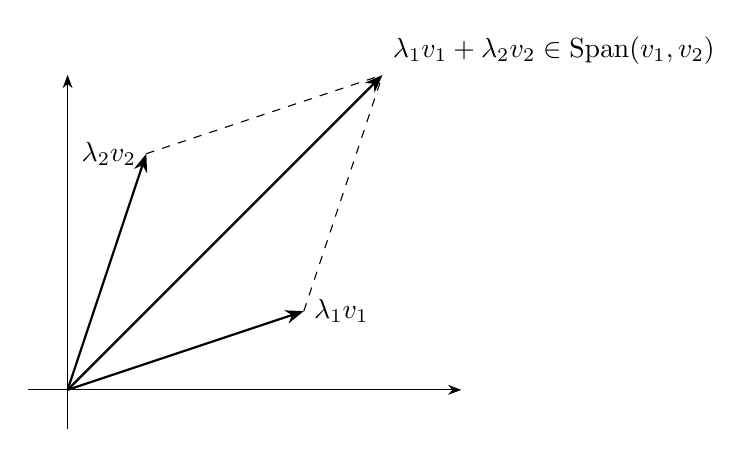
\begin{tikzpicture}[scale=1, >=Stealth]
\draw[->] (-0.5,0) -- (5,0);
\draw[->] (0,-0.5) -- (0,4);

\coordinate (v1) at (3,1);
\coordinate (v2) at (1,3);

\draw[->, thick] (0,0) -- (v1) node[right] {$\lambda_1 v_1$};
\draw[->, thick] (0,0) -- (v2) node[left] {$\lambda_2 v_2$};

\draw[dashed] (v1) -- ($(v1)+(v2)$);
\draw[dashed] (v2) -- ($(v1)+(v2)$);

\draw[->, thick] (0,0) -- ($(v1)+(v2)$) node[above right] {$\lambda_1 v_1+\lambda_2 v_2\in \operatorname{Span}(v_1,v_2)$};

\end{tikzpicture}
\end{center}
Furthermore, if \(v_1,v_2\) are linearly dependent, then \(\operatorname{Span}(v_1,v_2)\) is a line in \(\mathbb{R}^2\). For example, let \(v_1=\begin{pmatrix}2\\1\end{pmatrix}\) and
\(v_2=\begin{pmatrix}4\\2\end{pmatrix}\). Then \(v_2 = 2v_1\), so
\(\operatorname{Span}(v_1)=\operatorname{Span}(v_2)\). Geometrically, this is a straight line through the origin in the direction of \(v_1\) (and \(v_2\)). Let 
\[v_1=\begin{pmatrix}2\\1\end{pmatrix},\quad v_2=\begin{pmatrix}4\\2\end{pmatrix}.\]
Then \(v_2 = 2v_1\), so
\[\operatorname{Span}(v_1)=\operatorname{Span}(v_2).\]
\begin{center}
\begin{tikzpicture}[scale=1.1, >=Stealth]
\draw[->] (-3,0) -- (3,0);
\draw[->] (0,-3) -- (0,3);

\draw[thick] (-2.5,-1.25) -- (2.5,1.25);

\draw[->, thick] (0,0) -- (1,0.5) node[right] {$v_1$};
\draw[->, thick] (0,0) -- (2,1) node[right] {$v_2$};
\end{tikzpicture}
\end{center}

\paragraph{Span in $\mathbb{C}^n$}
The definition of span is the same in complex vector spaces, except the scalars are complex numbers.
\begin{definition}
The span over \(\mathbb{C}\) of vectors \(v_1,\ldots,v_n \in \mathbb{C}^n\) is
\[\operatorname{Span}_{\mathbb{C}}(v_1,\ldots,v_n) = \{\lambda_1 v_1 + \cdots + \lambda_n v_n : \lambda_i \in \mathbb{C}\}.\]
\end{definition}
Thus, \(\operatorname{Span}_{\mathbb{C}}(v_1,\ldots,v_n)\) consists of all vectors obtained by complex linear combinations of \(v_1,\ldots,v_n\).

\subsubsection{Standard Basis}
\begin{definition}[Standard basis of $\mathbb{R}^n$]
    The standard basis of \(\mathbb{R}^n\) is the set \(\{e_1,\ldots,e_n\}\), where
    \[e_1=\begin{pmatrix}1\\0\\\vdots\\0\end{pmatrix},\;e_2=\begin{pmatrix}0\\1\\\vdots\\0\end{pmatrix},\;\ldots,\;e_n=\begin{pmatrix}0\\0\\\vdots\\1\end{pmatrix}.\]
\end{definition}
\noindent Every vector \(x=\begin{pmatrix}x_1\\ \vdots \\ x_n\end{pmatrix}\in\mathbb{R}^n\) can be written uniquely as
\[x = x_1 e_1 + \cdots + x_n e_n.\]
We now verify that the standard basis really is a basis, by checking that it spans \(\mathbb{R}^n\) and is linearly independent.
\paragraph{Claim 1.}
The vectors \(e_1,\ldots,e_n\) span \(\mathbb{R}^n\).
\begin{proof}
    We show that any vector in \(\mathbb{R}^n\) can be written as a linear combination of \(e_1,\ldots,e_n\):
    \[\begin{pmatrix}x_1\\\vdots\\x_n\end{pmatrix} = \begin{pmatrix}x_1\\0\\\vdots\\0\end{pmatrix} + \begin{pmatrix}0\\x_2\\\vdots\\0\end{pmatrix} + \cdots + \begin{pmatrix}0\\\vdots\\0\\x_n\end{pmatrix} = x_1 e_1 + x_2 e_2 + \cdots + x_n e_n.\]
\end{proof}
\paragraph{Claim 2.}
The vectors \(e_1,\ldots,e_n\) are linearly independent.
\begin{proof}
    Suppose
    \[\lambda_1 e_1 + \cdots + \lambda_n e_n = 0.\]
    Then
    \[\begin{pmatrix}\lambda_1\\ \vdots \\ \lambda_n\end{pmatrix} = \begin{pmatrix}0\\ \vdots \\ 0\end{pmatrix},\]
    so \(\lambda_1=\cdots=\lambda_n=0\). Therefore \(e_1,\ldots,e_n\) are linearly independent.
\end{proof}
\medskip
\noindent
The standard basis also helps clarify the difference between real and complex vector spaces. In particular, the same vectors can generate very different spans depending on whether the scalars are real or complex.
\begin{example}[Standard basis and real vs complex span]
    Consider the standard basis \(e_1 = \begin{pmatrix}1\\0\end{pmatrix}, e_2 = \begin{pmatrix}0\\1\end{pmatrix}\) in \(\mathbb{C}^2\).
    \begin{itemize}
        \item Over \(\mathbb{C}\), any vector in \(\mathbb{C}^2\) can be written as
        \[z_1 e_1 + z_2 e_2, \quad z_1,z_2 \in \mathbb{C}.\]
        So the complex span is
        \[\operatorname{Span}_{\mathbb{C}}(e_1,e_2) = \mathbb{C}^2,\quad \dim_{\mathbb{C}} \mathbb{C}^2 = 2.\]

        \item Each complex scalar can be written as \(z_k = x_k + i y_k\), \(x_k,y_k \in \mathbb{R}\). Then
        \[z_1 e_1 + z_2 e_2 = x_1 e_1 + y_1 (i e_1) + x_2 e_2 + y_2 (i e_2),\]
        showing that every complex linear combination is also a real linear combination of the four vectors
        \[e_1, e_2, i e_1, i e_2.\]
        Hence, as a real vector space, \(\mathbb{C}^2\) has dimension 4:
        \[\dim_{\mathbb{R}} \mathbb{C}^2 = 4.\]
    \end{itemize}
    \begin{center}
    \begin{tikzpicture}[scale=1.2, >=Stealth]
    \draw[->] (-3,0) -- (3,0) node[right] {$\Re$};
    \draw[->] (0,-3) -- (0,3) node[above] {$\Im$};

    \draw[->, thick] (0,0) -- (2,0) node[below] {$1$};
    \draw[->, thick] (0,0) -- (0,2) node[left] {$i$};

    \node at (1.5,1.5) {$\mathbb{C}=\text{span}_{\mathbb{R}}(1,i)$};
    \end{tikzpicture}
    \end{center}
\end{example}


\subsection{Abstract Vector Spaces}
An abstract vector space generalizes the idea of vectors in \(\mathbb{R}^n\). It is a set equipped with two operations (vector addition and scalar multiplication) that satisfy certain rules (axioms).

\begin{definition}[Vector space over a field]
Let \(k\) be a field. A \textbf{vector space over \(k\)} is a set \(V\) together with two operations:
\[
v_1 + v_2 \in V, \quad \forall v_1,v_2 \in V, \qquad
\lambda v \in V, \quad \forall v \in V, \ \lambda \in k,
\]
satisfying the following axioms:
\begin{enumerate}
    \item Commutativity of addition: \(v_1 + v_2 = v_2 + v_1\)
    \item Associativity of addition: \((v_1 + v_2) + v_3 = v_1 + (v_2 + v_3)\)
    \item Existence of additive identity: \(\exists 0 \in V\) such that \(v + 0 = v\)
    \item Existence of additive inverses: \(\forall v \in V, \exists -v \in V\) with \(v + (-v) = 0\)
    \item Compatibility of scalar multiplication with field multiplication: \(\lambda(\mu v) = (\lambda\mu)v\)
    \item Identity element of scalar multiplication: \(1 v = v\)
    \item Distributivity of scalar multiplication over vector addition: \(\lambda(v_1 + v_2) = \lambda v_1 + \lambda v_2\)
    \item Distributivity of scalar multiplication over field addition: \((\lambda + \mu)v = \lambda v + \mu v\)
\end{enumerate}
\end{definition}

\begin{example}[Cartesian vector space]
Let \(K\) be a field. Then
\[
K^n = \left\{\begin{pmatrix}x_1\\\vdots\\x_n\end{pmatrix} : x_i \in K\right\}
\]
is a vector space over \(K\). Its standard basis is
\[
e_1 = \begin{pmatrix}1\\0\\\vdots\\0\end{pmatrix}, \dots, e_n = \begin{pmatrix}0\\\vdots\\0\\1\end{pmatrix},
\]
and \(\dim K^n = n\).
\end{example}

\begin{remark}[Span over integers is not a vector space]
\[
\operatorname{Span}_{\mathbb{Z}}(e_1,e_2) = \{\lambda_1 e_1 + \lambda_2 e_2 : \lambda_i \in \mathbb{Z}\}
\]
is an additive subgroup but not a vector space over \(\mathbb{R}\), because \(\mathbb{Z}\) is not a field.
\end{remark}

\begin{center}
\begin{tikzpicture}[scale=1.2, >=Stealth]
\draw[->] (-0.5,0) -- (3,0);
\draw[->] (0,-0.5) -- (0,3);

\draw[->, thick] (0,0) -- (2,0) node[below] {$e_1$};
\draw[->, thick] (0,0) -- (0,2) node[left] {$e_2$};

\node at (1.4,1.4) {$\mathbb{R}^2$};
\end{tikzpicture}
\end{center}

\subsubsection{Coordinate Spaces}
\marginpar{14 January, 2026}
\begin{definition}[Coordinate Spaces]
    A coordinate space of dimension \(n\) over a field \(k\) (\(k=\mathbb{R}\) or \(k=\mathbb{C}\)) is defined as
    \[k^n = \left\{\begin{pmatrix}x_1\\\vdots\\x_n\end{pmatrix} : x_i \in k\right\}.\]
    The standard basis is
    \[e_1=\begin{pmatrix}1\\0\\\vdots\\0\end{pmatrix}, \ \ldots \ , e_n=\begin{pmatrix}0\\\vdots\\0\\1\end{pmatrix}.\]
\end{definition}

\subsubsection{Polynomial Spaces}
\begin{definition}[Polynomial Spaces]
    A polynomial space of degree at most \(n\) over a field \(k\) is
    \[P_n(k) = \{ a_n x^n + \cdots + a_1 x + a_0 : a_i \in k \},\]
    which forms a vector space over \(k\).
\end{definition}
\begin{example}[Polynomial Spaces]
    Some examples of polynomials in these spaces are
    \[1+x^2 \in P_2(\mathbb{R}), \qquad 1+i x^3 \in P_3(\mathbb{C}).\]
    The subscript \(n\) indicates that \(\deg(f) \le n\).
    All polynomials can be collected in
    \[P_\infty = \{ a_n x^n + \cdots + a_1 x + a_0 : a_i \in k, \ n \ge 0 \},\]
    which is an infinite-dimensional vector space over \(k\).  
    We have the natural inclusions
    \[P_0 \subseteq P_1 \subseteq P_2 \subseteq \cdots \subseteq P_\infty.\]
    A standard basis for \(P_n(k)\) is 
    \[\{1, x, x^2, \ldots, x^n\},\]
    and every \(f \in P_n(k)\) can be written uniquely as
    \[f = \lambda_0 + \lambda_1 x + \lambda_2 x^2 + \cdots + \lambda_n x^n, \quad \lambda_i \in k.\]
\end{example}

\subsubsection{Matrix Spaces}
\begin{definition}[Matrix Spaces]
    The set of all \(n \times n\) matrices over a field \(k\) is
    \[M_n(k) = \left\{ \begin{pmatrix}
    a_{11} & \cdots & a_{1n} \\
    \vdots & \ddots & \vdots \\
    a_{n1} & \cdots & a_{nn}
    \end{pmatrix} : a_{ij} \in k \right\},\]
    which forms a vector space over \(k\).
    A standard basis for \(M_n(k)\) is the set of matrices \(\{ e_{ij} : 1 \le i,j \le n \}\), where \(e_{ij}\) has a 1 in the \((i,j)\)-th entry and 0 elsewhere.  
    The dimension is
    \[\dim M_n(k) = n^2.\]
\end{definition}
\begin{example}[Matrix Spaces]
    For \(M_2(\mathbb{R})\),
    \[\begin{pmatrix}1 & 2 \\ 3 & 4\end{pmatrix} = 1 e_{11} + 2 e_{12} + 3 e_{21} + 4 e_{22}.\]
\end{example}

\subsubsection{Function Spaces}
\marginpar{16 January, 2026}
\begin{definition}[Function spaces]
    Let $D$ be a set and $k$ a field. Define
    \[F(D,k) = \{ f : D \to k \}.\]
    With pointwise operations
    \[(f+g)(x) = f(x)+g(x), \quad (\lambda f)(x) = \lambda f(x),\]
    $F(D,k)$ is a vector space over $k$.
\end{definition}
\paragraph{1. Finite case: standard basis}
Assume $D = \{1,\dots,n\}$. For each $i \in D$, define the Kronecker delta function
\[\delta_i(j) = \begin{cases}1, & i=j,\\0, & i \ne j.\end{cases}\]
Then $\{\delta_1,\dots,\delta_n\}$ is a basis of $F(D,k)$. Moreover, every $f \in F(D,k)$ can be written uniquely as
\[f = \sum_{i=1}^n f(i)\,\delta_i.\]
Indeed, evaluating at $j$ gives
\[\sum_{i=1}^n f(i)\delta_i(j) = f(j),\]
so the functions span, and linear independence is immediate.
\paragraph{2. Infinite case}
If $D$ is infinite, $F(D,k)$ has no finite basis.  
The family $\{\delta_x : x \in D\}$ is linearly independent but does not span $F(D,k)$.

\subsection{Subspaces}
\marginpar{January 19, 2026}
\begin{definition}
    A subspace is a subset of a larger vector space that is itself a vector space, meaning it contains the zero vector and is closed under vector addition and scalar multiplication. Subspaces are essential because they allow focus on smaller, self-contained structures where standard linear algebra operations (like finding spans, bases, and transformations) still hold, with examples including lines through the origin in \(\mathbb{R}^{2}\), the null space of a matrix, or the entire space itself.
\end{definition}
\begin{proposition}[Subspace criterion]
    Let $V$ be a vector space over a field $k$ and let $U \subseteq V$. Then $U$ is a vector subspace of $V$ if and only if:
    \begin{enumerate}
    \item $0 \in U$,
    \item $u,v \in U \Rightarrow u+v \in U$,
    \item $u \in U,\ \lambda \in k \Rightarrow \lambda u \in U$.
    \end{enumerate}
\end{proposition}
\begin{problem}[Subspace criterion]
    Let $A \in M_n(K)$ be a fixed matrix. Prove thet
    \[U = \{x \in K^n : Ax = \vec{0}\}\]
    is a subspace, null space or kernel.
\end{problem}
\begin{problem}[Subspace criterion 2]
    Let $A \in M_n(K)$. Show that
    \[U = \{Ax : x \in K^n\}\]
    is a subspace of $K^n$. The set $U$ is called the image (or range) of $A$.
\end{problem}
\begin{problem}[Subspace criterion 3]
    Let $V = K$, viewed as a vector space over $K$. Show that the only subspaces of $V$ are $\{0\}$ and $V$ itself.
\end{problem}
\begin{problem}[Subspace criterion 4]
Let $V$ be a vector space over $K$ and let $v_1,\dots,v_n \in V$. Show that
\[\operatorname{Span}(v_1,\dots,v_n) = \{\lambda_1 v_1 + \cdots + \lambda_n v_n : \lambda_1,\dots,\lambda_n \in K\}\]
is a subspace of $V$.
\end{problem}

\marginpar{January 21, 2026}
\subsubsection{Membership in a span}
\begin{problem}[Span membership]
    Let
    \[v=\begin{pmatrix}3\\5\\-5\end{pmatrix},\quad v_1=\begin{pmatrix}1\\2\\1\end{pmatrix},\; v_2=\begin{pmatrix}2\\5\\4\end{pmatrix},\;
    v_3=\begin{pmatrix}1\\3\\6\end{pmatrix}.\]
    Decide whether $v \in \operatorname{Span}(v_1,v_2,v_3)$.
\end{problem}
\begin{problem}[Span membership 2]
    Let
    \[f = 3x^2 + 5x - 5,\quad f_1 = x^2 + 2x + 1,\; f_2 = 2x^2 + 5x + 4,\; f_3 = x^2 + 3x + 6.\]
    Decide whether $f \in \operatorname{Span}(f_1,f_2,f_3)$.
\end{problem}

\subsubsection{Operations on subspaces}
Let $W$ be a vector space and $U,V \subseteq W$ subspaces.
\begin{definition}[Intersection]
    \[U \cap V = \{w \in W : w \in U \text{ and } w \in V\}.\]
    The intersection of subspaces is a subspace. In particular, the smallest possible intersection is $\{0\}$.
\end{definition}
\begin{remark}
    In general, the union $U \cup V$ is not a subspace unless $U \subseteq V$ or $V \subseteq U$.
\end{remark}
\begin{definition}[Sum of subspaces]
    \[U + V = \{u+v : u \in U,\, v \in V\}.\]
\end{definition}
\begin{proposition}
    If $U$ and $V$ are subspaces of $W$, then $U+V$ is a subspace of $W$.
\end{proposition}
\begin{proof}[Proof that $U+V$ is a subspace]
    We apply the subspace criterion.
    (0) Since $0 \in U$ and $0 \in V$, we have $0 = 0+0 \in U+V$.
    (1) Let $w_1,w_2 \in U+V$. Then
    \[w_1=u_1+v_1,\quad w_2=u_2+v_2\]
    with $u_1,u_2 \in U$ and $v_1,v_2 \in V$. Hence
    \[w_1+w_2=(u_1+u_2)+(v_1+v_2) \in U+V.\]

    (2) Let $w \in U+V$ and $\lambda \in K$. Then $w=u+v$ and
    \[\lambda w=\lambda u+\lambda v \in U+V.\]
\end{proof}
\begin{proposition}
    \[U + V = \operatorname{Span}(U \cup V).\]
    Equivalently, $U+V$ is the smallest subspace of $W$ containing both $U$ and $V$.
\end{proposition}
\begin{proof}[Proof that $U+V = \operatorname{Span}(U \cup V)$]
    ($\subseteq$) Let $w \in U+V$. Then $w=u+v$ with $u \in U$, $v \in V$. Since $u,v \in U \cup V$, we have $w \in \operatorname{Span}(U \cup V)$.

    ($\supseteq$) Let $w \in \operatorname{Span}(U \cup V)$. Then
    \[w = a_1u_1 + \cdots + a_nu_n + b_1v_1 + \cdots + b_mv_m\]
    with $u_i \in U$, $v_j \in V$. Grouping terms,
    \[w = (a_1u_1 + \cdots + a_nu_n) + (b_1v_1 + \cdots + b_mv_m),\]
    so $w \in U+V$.
\end{proof}

\subsection{Direct sums}
\marginpar{January 23, 2026}
Let $W$ be a vector space and $U,V \subseteq W$ subspaces.
\begin{definition}[Direct sum]
    We say that $U$ and $V$ are in direct sum if
    \[U \cap V = \{0\}.\]
    In this case, their sum
    \[U+V=\{u+v : u \in U,\; v \in V\}\]
    is denoted by $U \oplus V$.
    We write
    \[W = U \oplus V\]
    if and only if
    \[\begin{cases}
    W = U+V,\\
    U \cap V = \{0\}.
    \end{cases}\]
\end{definition}
\begin{remark}
    To prove $W = U \oplus V$, one must show:
    \begin{itemize}
    \item Every $w \in W$ can be written as $w=u+v$ with $u \in U$, $v \in V$.
    \item If $w \in U$ and $w \in V$, then $w=0$.
    \end{itemize}
\end{remark}
\subsubsection*{Analogy with sets}
\[\begin{array}{c|c}
\text{Sets} & \text{Vector spaces} \\
\hline
A \cap B & U \cap V \\
A \cup B & U + V \\
A \sqcup B,\ A \cap B = \emptyset & U \oplus V,\ U \cap V = \{0\}
\end{array}\]
\begin{example}
    Let
    \[D=\{1,2,3,4,5\},\quad A=\{1,2,3\},\quad B=\{4,5\}.\]
    Then
    \[D = A \sqcup B.\]
\end{example}

\subsubsection{Direct sums in function spaces}
Let $D$ be a set and $A \subseteq D$. Consider the function space $F(D,\mathbb{R})$.
\begin{definition}[]
    Define
    \[U = \{f \in F(D,\mathbb{R}) : f(x)=0 \text{ for all } x \notin A\}.\]
    Then $U$ is a subspace of $F(D,\mathbb{R})$, and $U$ can be identified with $F(A,\mathbb{R})$.
\end{definition}
\begin{remark}
    Every function in $U$ is completely determined by its values on $A$ and vanishes outside $A$.
\end{remark}

\section{Basis and Dimension}
\marginpar{January 26, 2026}
\subsection{Finite Dimensional Spaces}
Let V be a vector space over a field k. Then there are two possibilities:
\begin{itemize}
    \item The zero vector space: $V = \{0\}$
    \item The non-zero vector space: $V \neq \{0\}$
\end{itemize}
In the second case, there exists a non-zero vector $v_1 \in V$ such that $v_1 \neq 0$. Then $span(v_1)$ is a subspace of $V$, and there are two possibilities:
\begin{itemize}
    \item $V = span(v_1)$, i.e., $v_1$ is a generator of $V$.
    \item $V \neq span(v_1)$, i.e., there exists a $v_2 \in V$ such that $v_2 \notin span(v_1)$.
\end{itemize}
In the second case, $span(v_1,v_2) \subseteq V$. This process can be repeated to obtain a sequence of vectors $v_1,v_2,\ldots,v_n$ such that $span(v_1,\ldots,v_n) \subseteq V$. The maximum number of linearly independent vectors in $V$ is called the dimension of $V$, denoted by $\dim V$.

2 cases (2d space plane):
\begin{itemize}
    \item $v = v_2 = span(v_1,v_2)$
    \item $v \neq v_2 \quad \exists v_3 \notin v_2$, where $v_3 = span(v_1,v_2,v_3) \subseteq v$
\end{itemize}

2 cases (3d space):
\begin{itemize}
    \item $v_3 = v$
    \item $v_3 \neq v \quad \exists v_4...$
\end{itemize}
\begin{definition}
    $V$ is finite dimensional if it can be spanned by finitely many vectors.
    \[\exists v_1,\ldots,v_n : V = span(v_1,\ldots,v_n).\]
    $dim V =$ smallest $n$ such that $V = span(v_1,\ldots,v_n)$.
\end{definition}
$dim_kV =$ min $n$ such that $V = span_k(v_1,\ldots,v_n)$.
\begin{example}
    $(\mathbb{C}^n,n=1)$
    $\mathbb{C} = span_{\mathbb{R}}(1,i) = 2$
    \[x \cdot 1 + y \cdot i\]
    $M_n(\mathbb{C})$
    \[A = \begin{pmatrix}
        z_{11} & z_{12} & \cdots & z_{1n}\\
        \vdots & \vdots & \ddots & \vdots\\
        z_{n1} & z_{n2} & \cdots & z_{nn}
    \end{pmatrix} = \begin{pmatrix}
        x_{11} + y_{11}i & x_{12} + y_{12}i & \cdots & x_{1n} + y_{1n}i\\
        \vdots & \vdots & \ddots & \vdots\\
        x_{n1} + y_{n1}i & x_{n2} + y_{n2}i & \cdots & x_{nn} + y_{nn}i
    \end{pmatrix}\]
    First matrix is of $dim_{\mathbb{C}}M_n(\mathbb{C}) = n^2$, and the second matrix is of $dim_{\mathbb{R}}M_n(\mathbb{C}) = 2n^2$.
\end{example}
\begin{example}[dim $V = \infty$]
    \[P_{\infty}\]
    \[v_1 = 1 \quad v_2 = x \quad v_3 = x^2\]
    $span(v_1) =$ constant polynomials
    \[V_1 = span(v_1,v_2) = P_1\]
    \[v_{n+1} = x^n \notin P_{n-1}\]
\end{example}

\subsection{Linear Independence}
\begin{definition}
    $v_1,\ldots,v_n$ are linearly independent if $\lambda_1v_1 + \ldots + \lambda_nv_n = 0 \implies \lambda_1 = \ldots = \lambda_n = 0$.
\end{definition}
\begin{example}
    \[e_1 = \begin{pmatrix}
        1\\0
    \end{pmatrix} \quad e_2 = \begin{pmatrix}
        0\\1
    \end{pmatrix}\]
    Prove LI.
    Assume $xe_1 + ye_2 = 0$. Prove $x=y=0$.
    \[xe_1 + ye_2 = x\begin{pmatrix}
        1\\0
    \end{pmatrix} + y\begin{pmatrix}
        0\\1
    \end{pmatrix} = \begin{pmatrix}
        x\\y
    \end{pmatrix} = 0 \implies x = y = 0.\]
\end{example}
\begin{proposition}
    The "standard basis" are both spanning and LI.
    $(e_1,\ldots,e_n)$ of $k^n$
    $(1,x,\ldots,x^{n})$ of $P_n$
    $(e_{11},\ldots,e_{nn})$ of $M_n(k)$
    $(\delta_1,\ldots,\delta_n)$ of $F(D)$, where $D = \{1,\ldots,n\}$
\end{proposition}
\begin{definition}
    basis $= set(v_1,\ldots,v_n)$ both span and LI.
    \[dim(\forall) = \#basis\]
\end{definition}
\begin{problem}
    Prove $dim P_{\infty} = \infty$.
    Assume $dim P_{\infty} < \infty$. Proof by contradiction.
    $\exists f_1,\ldots,f_n$ polynomials $P_{\infty}=span(f_1,\ldots,f_n)$. Let $d =$ max degree of $f_k$.
    \[x^{d+1} \notin span(f_1,\ldots,f_n)\]
    degree $\leq d$.
\end{problem}

\marginpar{January 28, 2026}
\begin{problem}
    \[v_1 = \begin{pmatrix}1\\1\\0\end{pmatrix}, \quad v_2 = \begin{pmatrix}1\\3\\2\end{pmatrix}, \quad v_3 = \begin{pmatrix}4\\9\\5\end{pmatrix}.\]
    Are these vectors linearly independent? Are there $x,y,z \in \mathbb{R}$ such that 
    \[xv_1 + yv_2 + zv_3 = 0?\]
\end{problem}
\begin{solution}
    $x,y,z$ not all zero.
    \[x\begin{pmatrix}1\\1\\0\end{pmatrix} + y\begin{pmatrix}1\\3\\2\end{pmatrix} + z\begin{pmatrix}4\\9\\5\end{pmatrix} = \begin{pmatrix}0\\0\\0\end{pmatrix}\]
    \[\begin{cases}x + 3y + 4z = 0\\1 + 3y + 9z = 0\\0 + 2y + 5z = 0\end{cases}\]
    Find a non-trivial solution. $x = 3$, $y = 5$, $z = -2$. Not LI: $3v_1 + 5v_2 - 2v_3 = 0$.
\end{solution}
\begin{definition}[Linear Dependence]
    Linearly dependent (LD) just means not LI.
\end{definition}
\begin{proposition}
    $v_1,\ldots,v_n$ are linearly dependent if and only if one vector is in the span of the other vectors.
\end{proposition}
\begin{example}
    \[3v_1 + 5v_2 - 2v_3 = 0\]
    As we can see, $v_1$ is in the span of $v_2$ and $v_3$.
    \[v_1 = \frac{1}{3}(-5v_2+2v_3)\]
\end{example}
\begin{remark}
    If one vector $v_1 = 0$ then the family is LD.
\end{remark}
\begin{proof}
    Proof of $\longrightarrow$: Assumption  $\lambda_1v_1 + \cdots + \lambda_nv_n = 0$. Not all $\lambda_i$ are zero, at least one is nonzero, say $\lambda_k \neq 0$.
    The goal is to write $v_k$ in the span of the other vectors.
    \[v_k = \frac{-1}{\lambda_k}\sum_{i \neq k} \lambda_iv_i.\]
    \[v_k \in span(v_1,\ldots,v_k,\ldots,v_n).\]

    Converse: Assume one vector, say $v_k$ is in the span of the other vectors.
    \[v_k \in span(v_1,\ldots,v_k,\ldots,v_n).\]
    There exists coefficients $\lambda_1,\ldots,\lambda_n$ such that
    \[v_k = \lambda_1v_1 + \cdots + \lambda_{k-1}v_{k+-1} + \lambda_{k+1}v_{k+1} + \cdots + \lambda_nv_n.\]
    LD: non trivial dependency between the $v_i$'s.
\end{proof}
\begin{example}
    \[V = \mathbb{R}^3\]
    \[v_1 = \begin{pmatrix}a_1\\0\\0\end{pmatrix}, \quad v_2 = \begin{pmatrix}b_1\\b_2\\0\end{pmatrix}, \quad v_3 = \begin{pmatrix}c_1\\c_2\\c_3\end{pmatrix}.\]
    LI:
    \[v_1 = \begin{pmatrix}1\\0\\0\end{pmatrix}, \quad v_2 = \begin{pmatrix}1\\2\\0\end{pmatrix}, \quad v_3 = \begin{pmatrix}1\\2\\3\end{pmatrix}.\]
    LD:
    \[v_1 = \begin{pmatrix}1\\0\\0\end{pmatrix}, \quad v_2 = \begin{pmatrix}1\\2\\0\end{pmatrix}, \quad v_3 = \begin{pmatrix}1\\3\\0\end{pmatrix}.\]

    Assume $xv_1 + yv_2 + zv_3 = 0$.
    \[x\begin{pmatrix}a_1\\0\\0\end{pmatrix} + y\begin{pmatrix}b_1\\b_2\\0\end{pmatrix} + z\begin{pmatrix}c_1\\c_2\\c_3\end{pmatrix}.\]

    \[\begin{cases}
        a_1x + b_1y + c_1z = 0\\
        b_2y + c_2z = 0\\
        c_3z = 0
    \end{cases}\]

    If $a_1 = 0$. $v_1 = \begin{pmatrix}0\\0\\0\end{pmatrix}$. Answer: LD. Can assume $a_1 \neq 0$.
    If $b_2 = 0$. $v_1 = \begin{pmatrix}a_1\\0\\0\end{pmatrix}, \quad v_2 = \begin{pmatrix}b_1\\0\\0\end{pmatrix}$. Answer: LD.
\end{example}


\section{Appendix}

\section{Solutions}

\begin{solution}[Invertibility]
    Suppose \(B\) and \(B'\) are both inverses of \(A\). Then
    \[B = B I = B(AB') = (BA)B' = I B' = B'.\]
    Therefore, \(B = B'\), so the inverse is unique.
\end{solution}
\begin{solution}[Invertibility 2]
    We can answer this problem with proof by contradiction. Let's
    suppose this matrix is invertible. By definition there exists B = $\begin{pmatrix}a&b\\c&d\end{pmatrix}$ such that $\begin{bmatrix}0&1\\0&0\end{bmatrix}$ $\begin{bmatrix}a&b\\c&d\end{bmatrix}$ = $\begin{bmatrix}1&0\\0&1\end{bmatrix}$.  We can rewrite this equation into: $\begin{bmatrix}a&b\\c&d\end{bmatrix}$ = $\begin{bmatrix}0&1\\0&0\end{bmatrix}^{-1}$. The inverse of our matrix can be rewritten as $\frac{1}{0*0 - 1*0}\begin{bmatrix}0&-1\\0&0\end{bmatrix}$\footnote{Recall that an inverse of a $2 \times 2$ matrix is equal to its determinant multiplied with its conjugate}. But this is undefined since division by 0 is undefined. Therefore, our initial assumption that the matrix is invertible is false, and thus the matrix is not invertible.
\end{solution}
\begin{solution}[Field]
    A field with 2 elements can be constructed as follows:
    Let \(F = \{0, 1\}\) be a set with two elements. We define addition and multiplication operations on \(F\) as follows:
    \begin{itemize}
        \item \(0 + 0 = 0\)
        \item \(0 + 1 = 1\)
        \item \(1 + 0 = 1\)
        \item \(1 + 1 = 0\)
        \item \(0 \times 0 = 0\)
        \item \(0 \times 1 = 0\)
        \item \(1 \times 0 = 0\)
        \item \(1 \times 1 = 1\)
    \end{itemize}
\end{solution}
\begin{solution}[Span]
    \[\operatorname{Span}(v_1,v_2) = \{xv_1 + yv_2 : x,y \in \mathbb{R}\} = \left\{\begin{pmatrix}3x + y\\x + 3y\end{pmatrix}: x,y \in \mathbb{R}\right\}.\]
\end{solution}
\begin{solution}[Subspace Criterion]
    Let $A \in M_n(K)$ be fixed and define
    \[U = \{x \in K^n : Ax = \vec{0}\}.\]
    We verify the subspace criterion.

    (0) Non-empty:  
    Since $A0 = 0$, we have $0 \in U$.

    (1) Closed under addition:  
    Let $x,y \in U$. Then $Ax = 0$ and $Ay = 0$. Hence
    \[A(x+y) = Ax + Ay = 0 + 0 = 0,\]
    so $x+y \in U$.

    (2) Closed under scalar multiplication:  
    Let $x \in U$ and $\lambda \in K$. Then
    \[A(\lambda x) = \lambda Ax = \lambda 0 = 0,\]
    so $\lambda x \in U$.

    Therefore, by the subspace criterion, $U$ is a subspace of $K^n$. It is called the null space (kernel) of $A$.
\end{solution}
\begin{solution}[Subspace Criterion 2]
    We verify the subspace criterion.

    (0) Non-empty:  
    Since $A0 = 0$, we have $0 \in U$.

    (1) Closed under addition:  
    Let $y_1,y_2 \in U$. Then there exist $x_1,x_2 \in K^n$ such that
    \[y_1 = Ax_1, \quad y_2 = Ax_2.\]
    Hence,
    \[y_1 + y_2 = Ax_1 + Ax_2 = A(x_1 + x_2) \in U.\]

    (2) Closed under scalar multiplication:  
    Let $y \in U$ and $\lambda \in K$. Then $y = Ax$ for some $x \in K^n$, and
    \[\lambda y = \lambda Ax = A(\lambda x) \in U.\]

    Therefore, by the subspace criterion, $U$ is a subspace of $K^n$. It is called the image of $A$.
\end{solution}
\begin{solution}[Subspace Criterion 3]
    Let $U \subseteq K$ be a subspace. We show that either $U = \{0\}$ or $U = K$. If $U = \{0\}$, we are done. Otherwise, $U \neq \{0\}$. Then there exists $v \in U$ with $v \neq 0$.
    We prove that $U = K$. Let $x \in K$ be arbitrary. Since $v \neq 0$, there exists $\lambda \in K$ such that
    \[x = \lambda v.\]
    Because $U$ is closed under scalar multiplication, $\lambda v \in U$, hence $x \in U$. Therefore every $x \in K$ belongs to $U$, so $U = K$. Conclusion: the only subspaces of $K$ are $\{0\}$ and $K$.
\end{solution}
\begin{solution}[Subspace Criterion 4]
    We verify the subspace criterion.
    (0) Non-empty:  
    Taking $\lambda_1=\cdots=\lambda_n=0$ gives
    \[0 = 0v_1 + \cdots + 0v_n \in \operatorname{Span}(v_1,\dots,v_n).\]
    (1) Closed under addition:  
    Let $u,v \in \operatorname{Span}(v_1,\dots,v_n)$. Then there exist scalars
    $a_1,\dots,a_n,b_1,\dots,b_n \in K$ such that
    \[u = a_1 v_1 + \cdots + a_n v_n, \quad v = b_1 v_1 + \cdots + b_n v_n.\]
    Hence,
    \[u+v = (a_1+b_1)v_1 + \cdots + (a_n+b_n)v_n \in \operatorname{Span}(v_1,\dots,v_n).\]
    (2) Closed under scalar multiplication:  
    Let $u \in \operatorname{Span}(v_1,\dots,v_n)$ and $\lambda \in K$. Then
    \[u = a_1 v_1 + \cdots + a_n v_n\]
    for some scalars $a_i$, and
    \[\lambda u = (\lambda a_1)v_1 + \cdots + (\lambda a_n)v_n \in \operatorname{Span}(v_1,\dots,v_n).\]
    Therefore, $\operatorname{Span}(v_1,\dots,v_n)$ is a subspace of $V$.
\end{solution}
\begin{solution}[Span Membership]
    We look for scalars $x,y,z \in \mathbb{R}$ such that
    \[xv_1 + yv_2 + zv_3 = v.\]
    That is,
    \[x\begin{pmatrix}1\\2\\1\end{pmatrix} + y\begin{pmatrix}2\\5\\4\end{pmatrix} + z\begin{pmatrix}1\\3\\6\end{pmatrix} = \begin{pmatrix}3\\5\\-5\end{pmatrix}.\]
    This gives the system
    \[\begin{cases}
    x + 2y + z = 3,\\
    2x + 5y + 3z = 5,\\
    x + 4y + 6z = -5.
    \end{cases}\]
    Solving, we obtain
    \[x=3,\quad y=1,\quad z=-2.\]
    Therefore,
    \[v = 3v_1 + v_2 - 2v_3,\]
    so $v \in \operatorname{Span}(v_1,v_2,v_3)$.
\end{solution}
\begin{solution}[Span Membership 2]
    We seek scalars $x,y,z \in \mathbb{R}$ such that
    \[f = xf_1 + yf_2 + zf_3.\]
    Comparing coefficients,
    \[x(x^2+2x+1) + y(2x^2+5x+4) + z(x^2+3x+6) = 3x^2+5x-5,\]
    which gives
    \[\begin{cases}
    x + 2y + z = 3,\\
    2x + 5y + 3z = 5,\\
    x + 4y + 6z = -5.
    \end{cases}\]
    Solving,
    \[x=3,\quad y=1,\quad z=-2.\]
    Hence,
    \[f = 3f_1 + f_2 - 2f_3,\]
    and therefore $f \in \operatorname{Span}(f_1,f_2,f_3)$.
\end{solution}

\section{Useful Links}

\end{document}